\chapter{Training Results}\label{app:training_results}
\begin{figure}[htbp!]
    \centering
    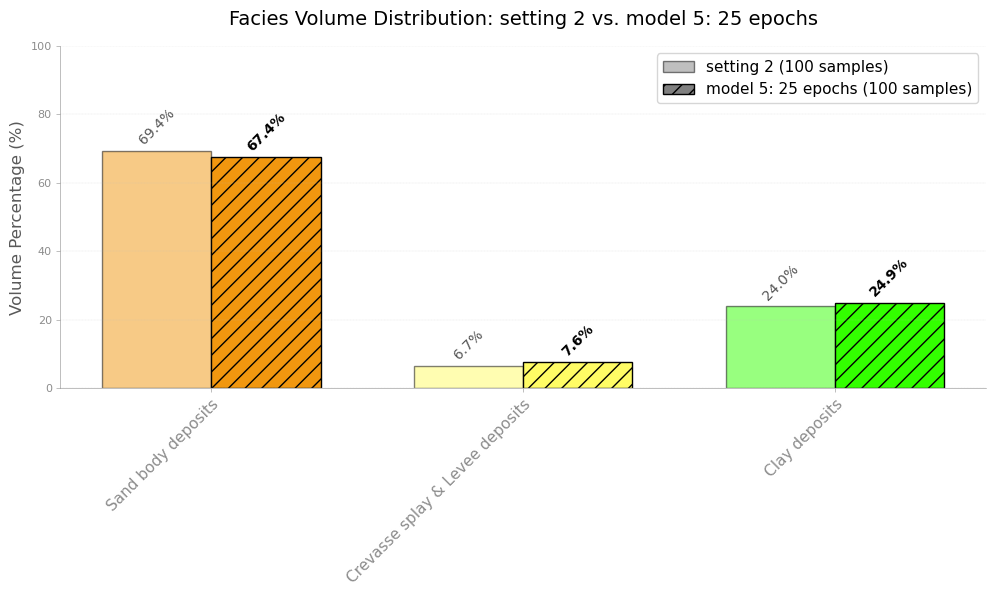
\includegraphics[width=0.8\linewidth]{figures/appendix/appendix_F/facies_distribution_model_5_setting_2.png}
    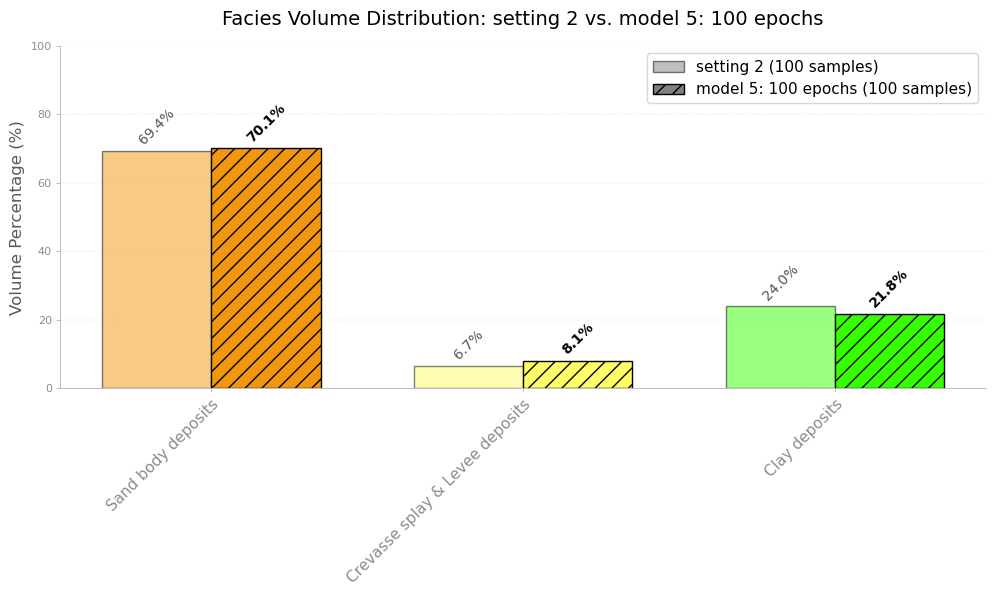
\includegraphics[width=0.8\linewidth]{figures/appendix/appendix_F/facies_distribution_model_5_1_setting_2.png}
    \caption{Comparison of global categorical facies distributions between the training dataset and Models 5 \& 5.1.}
    \label{fig:facies_dist_unconstrained_model}
\end{figure}

\begin{figure}[ht]
    \centering
    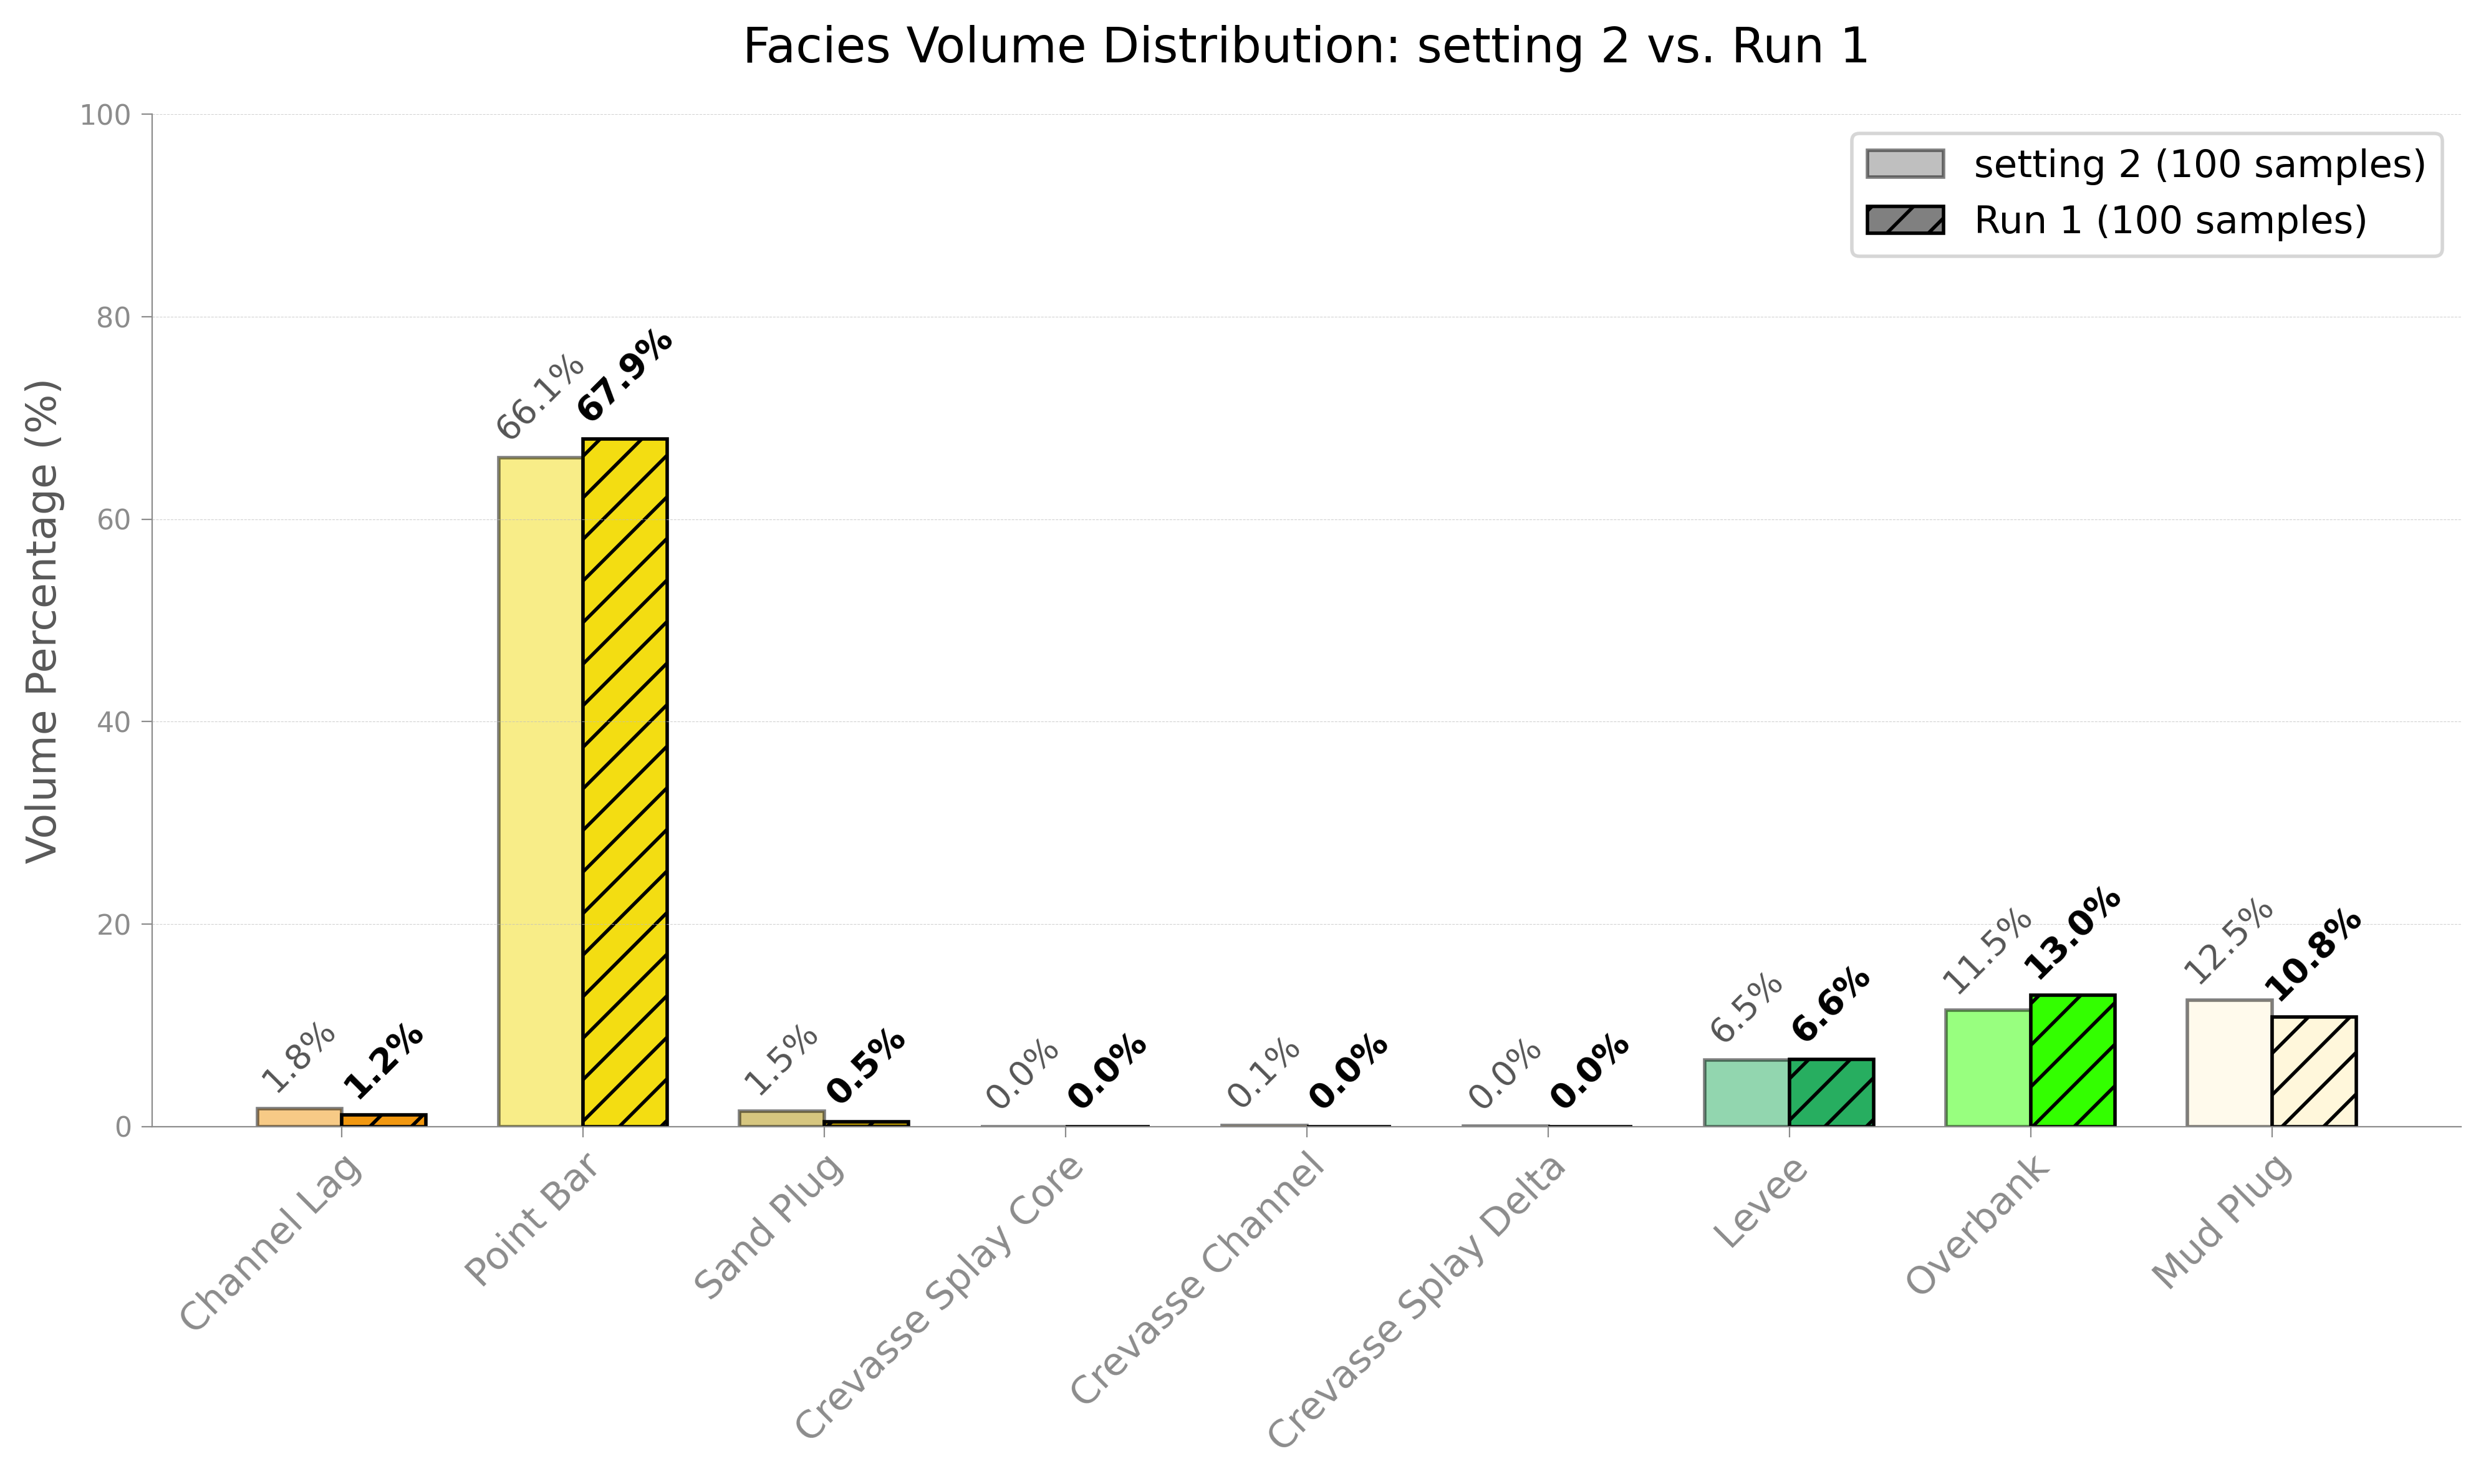
\includegraphics[width=0.9\textwidth]{figures/appendix/appendix_F/facies_distribution_hf.png}
    \caption{Global categorical facies distribution comparison between the high-fidelity model and the training dataset.}
    \label{fig:app_facies_dist_high_fidelity_model}
\end{figure}

\begin{figure}[ht]
    \centering
    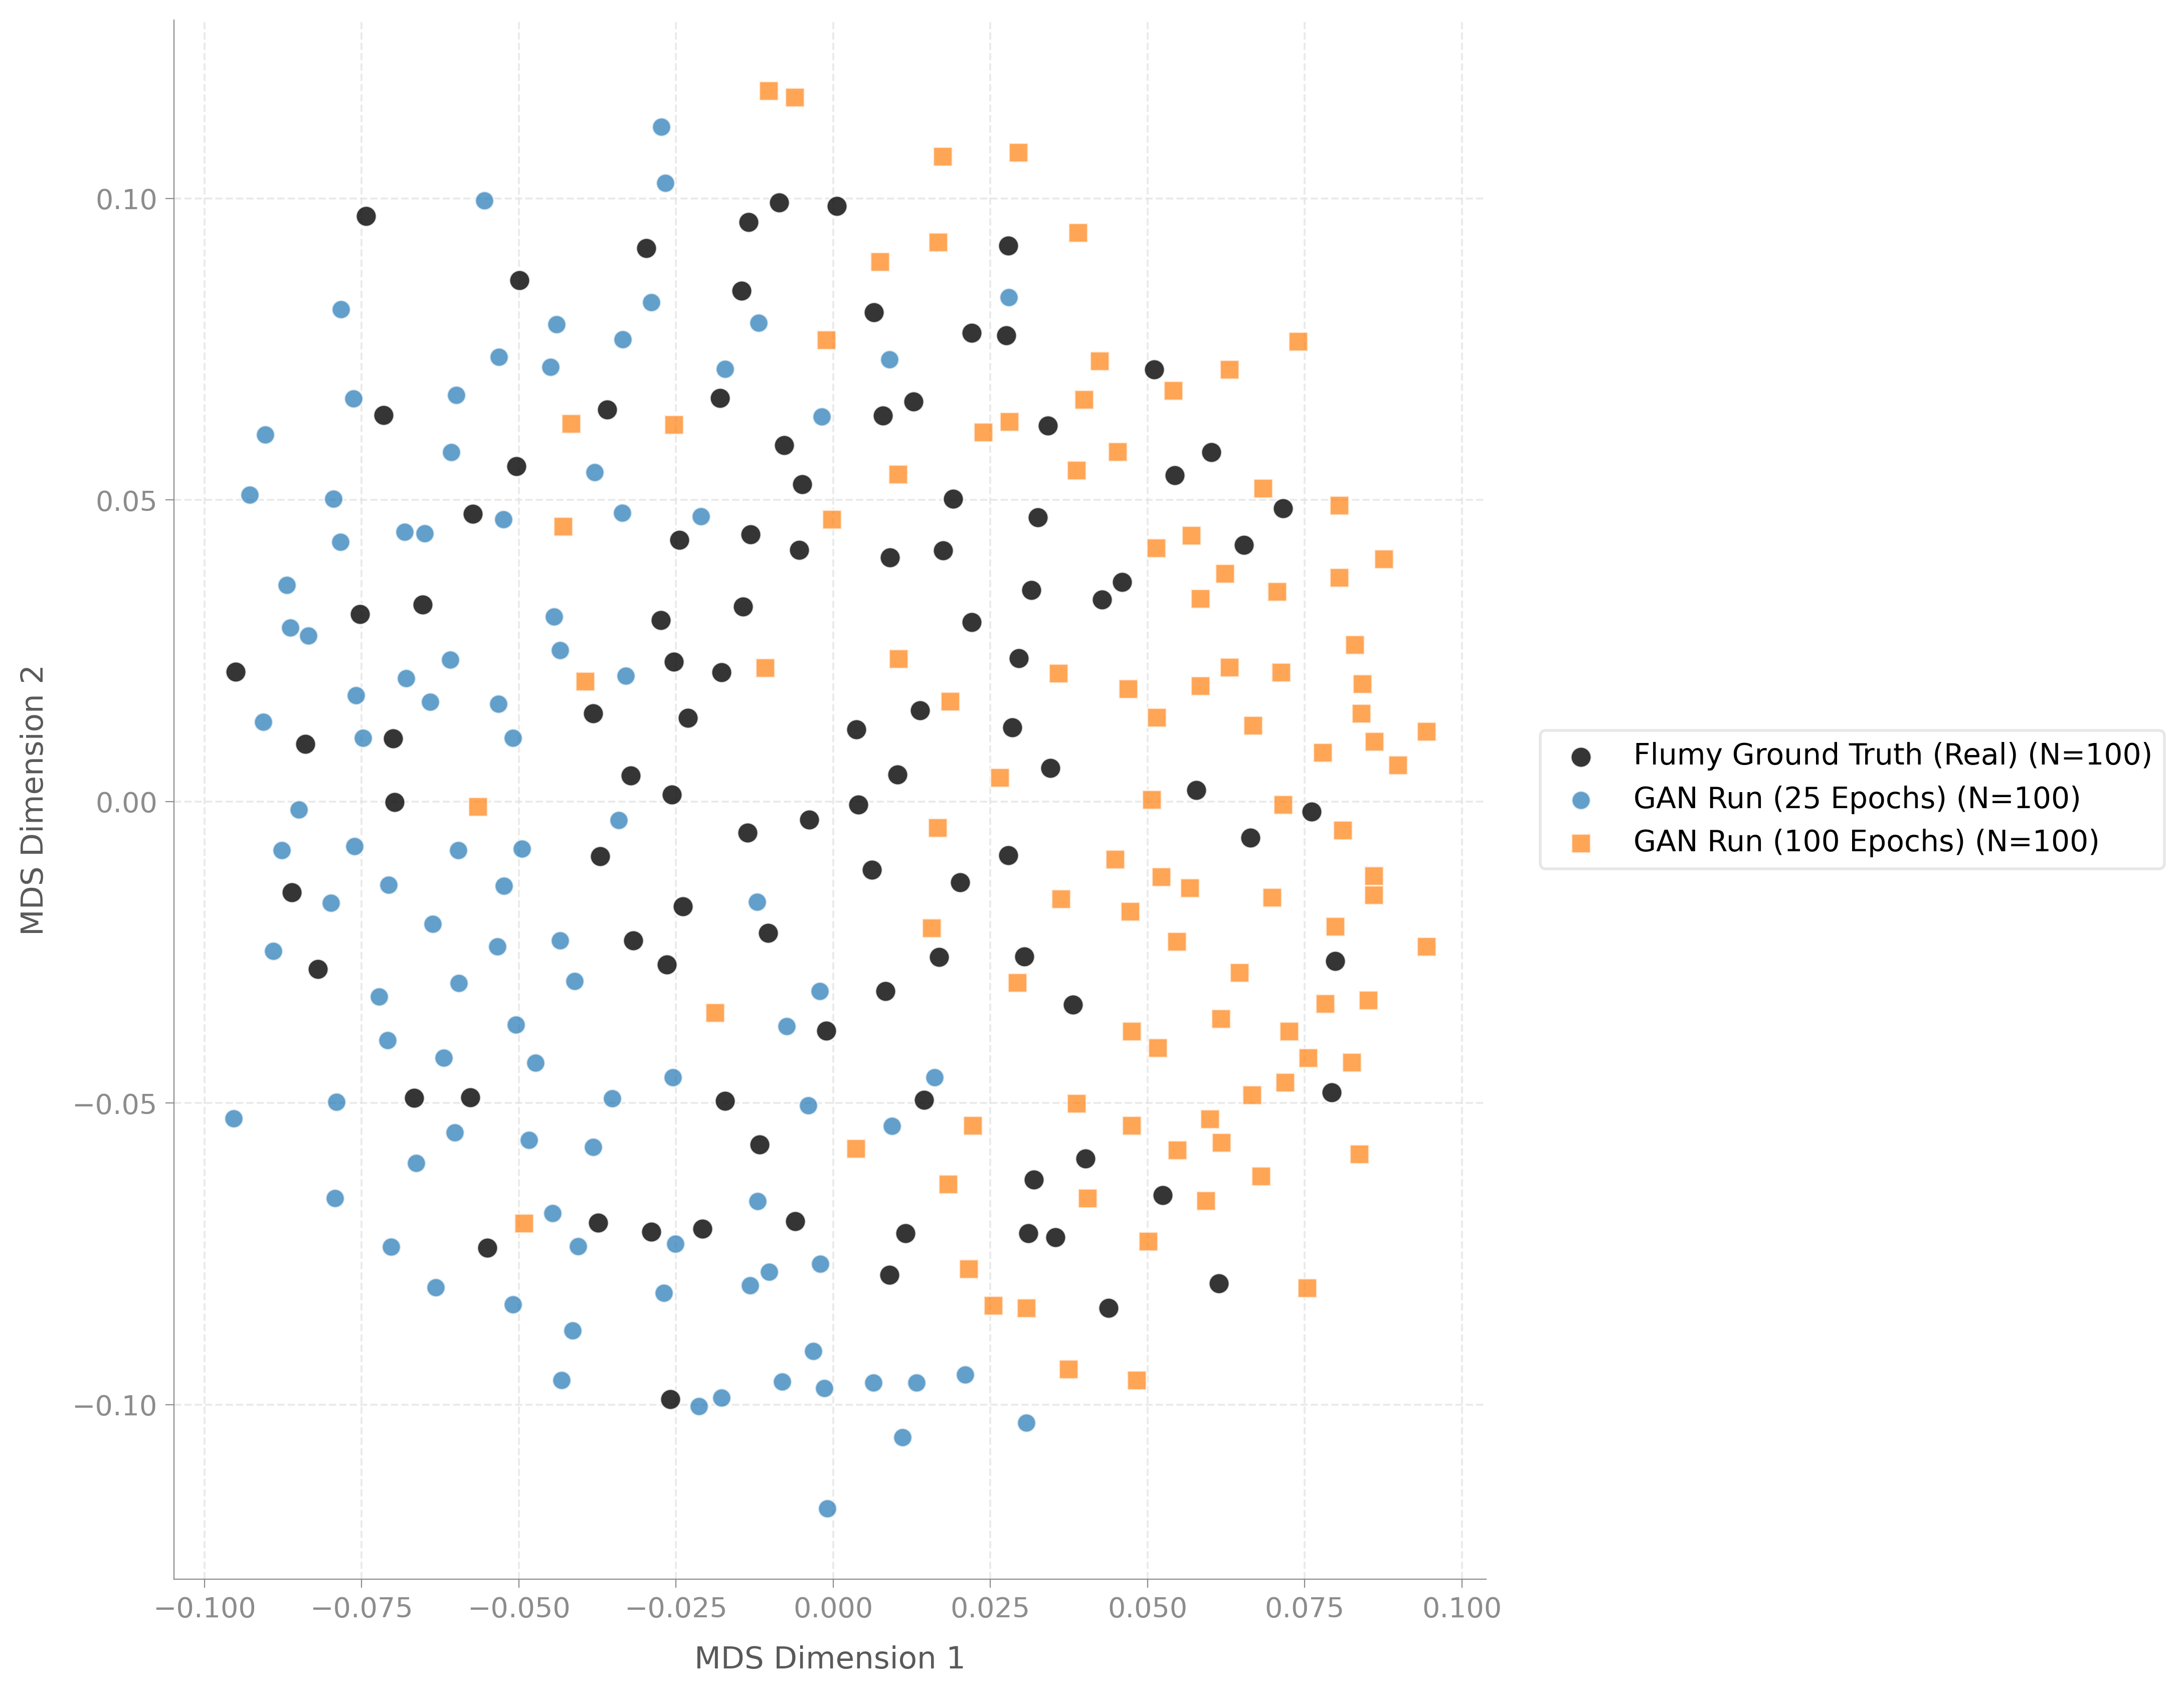
\includegraphics[width=0.9\textwidth]{figures/results/cgan_unconstrained_performance/ms_swd_mds_plot.png}
    \caption{2D~\gls{mds} comparison plot between setting 2, and Models 5 \& 5.1.}
    \label{fig:2d_mds_unconstrained_models_5_and_5_1}
\end{figure}



\begin{figure}[ht]
    \centering
    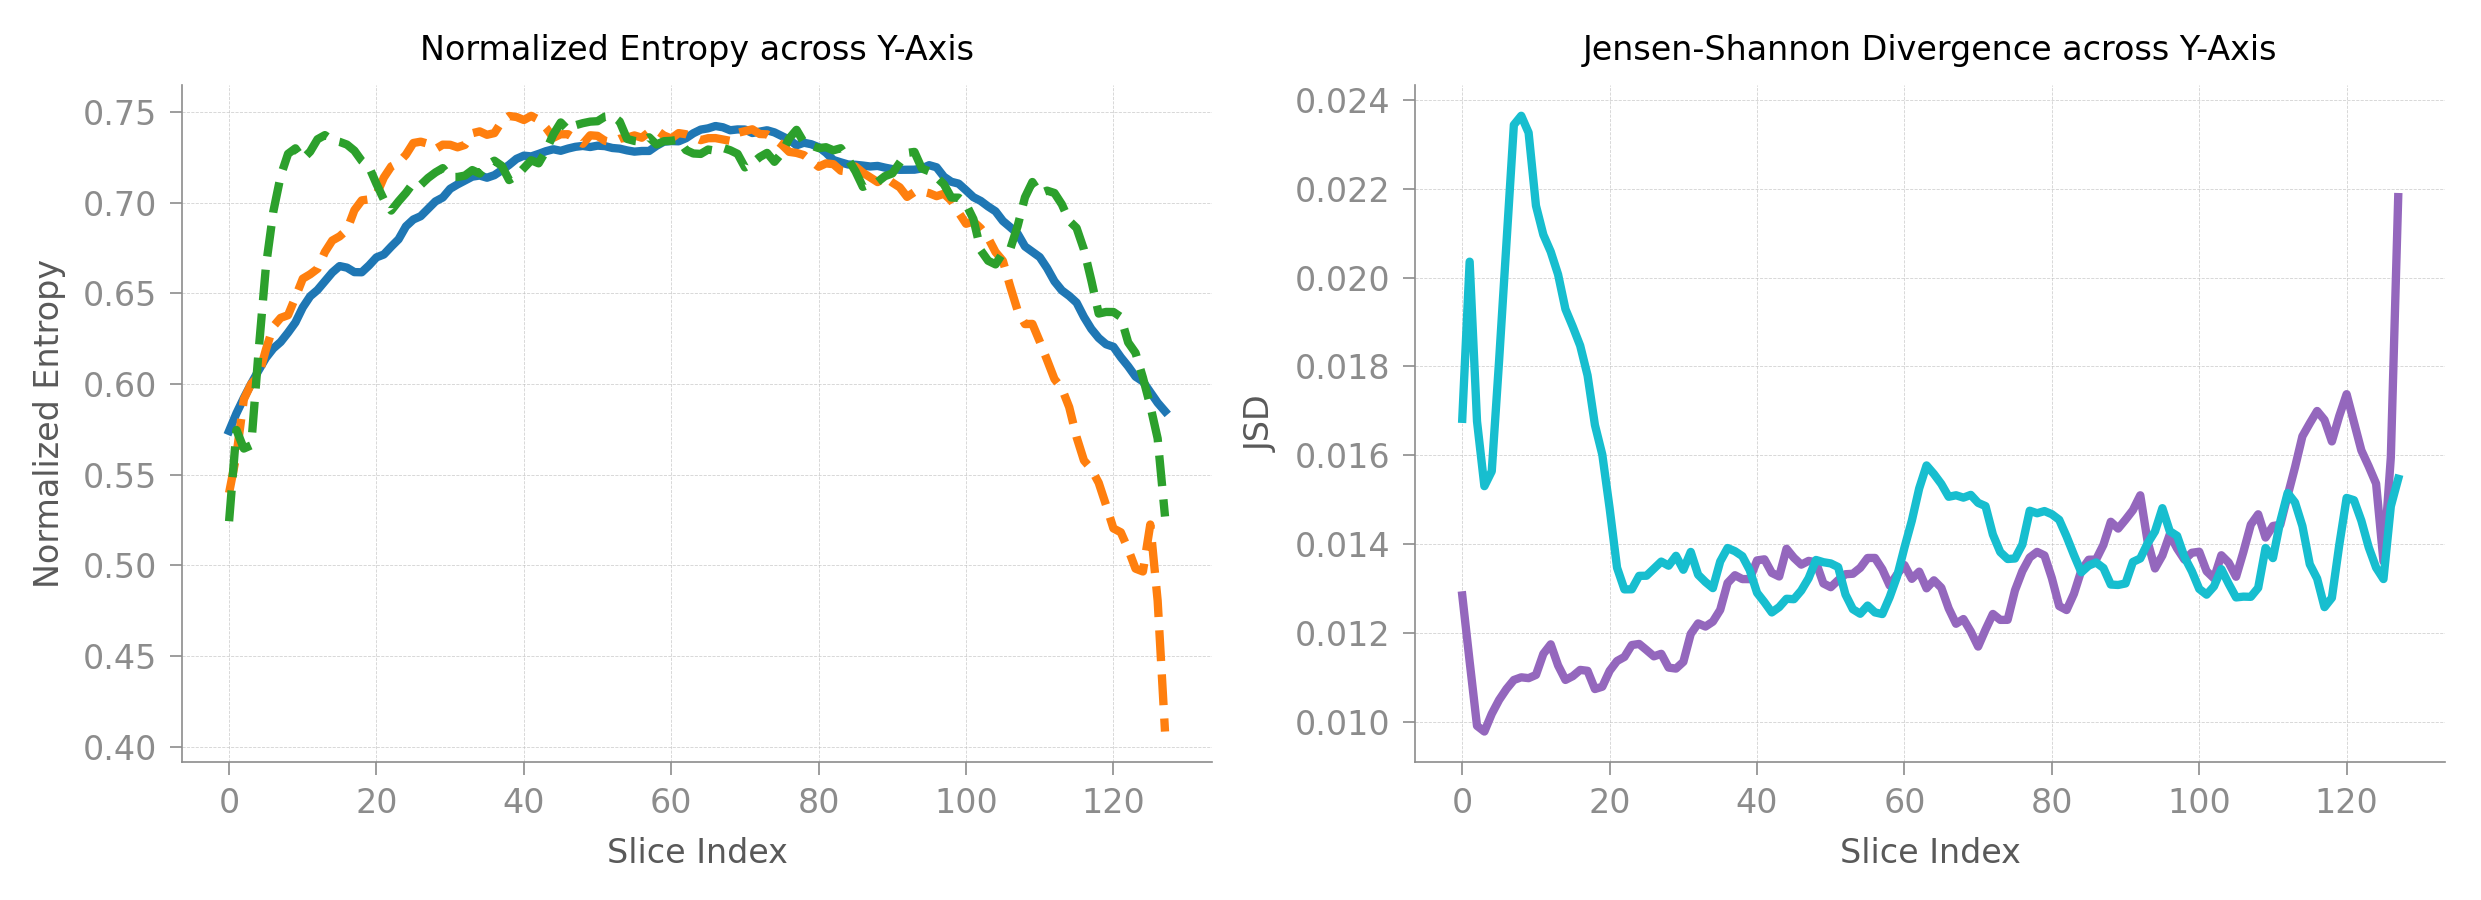
\includegraphics[width=0.9\textwidth]{figures/results/cgan_unconstrained_performance/combined_H_and_JSD_metrics_axis_Y.png}
    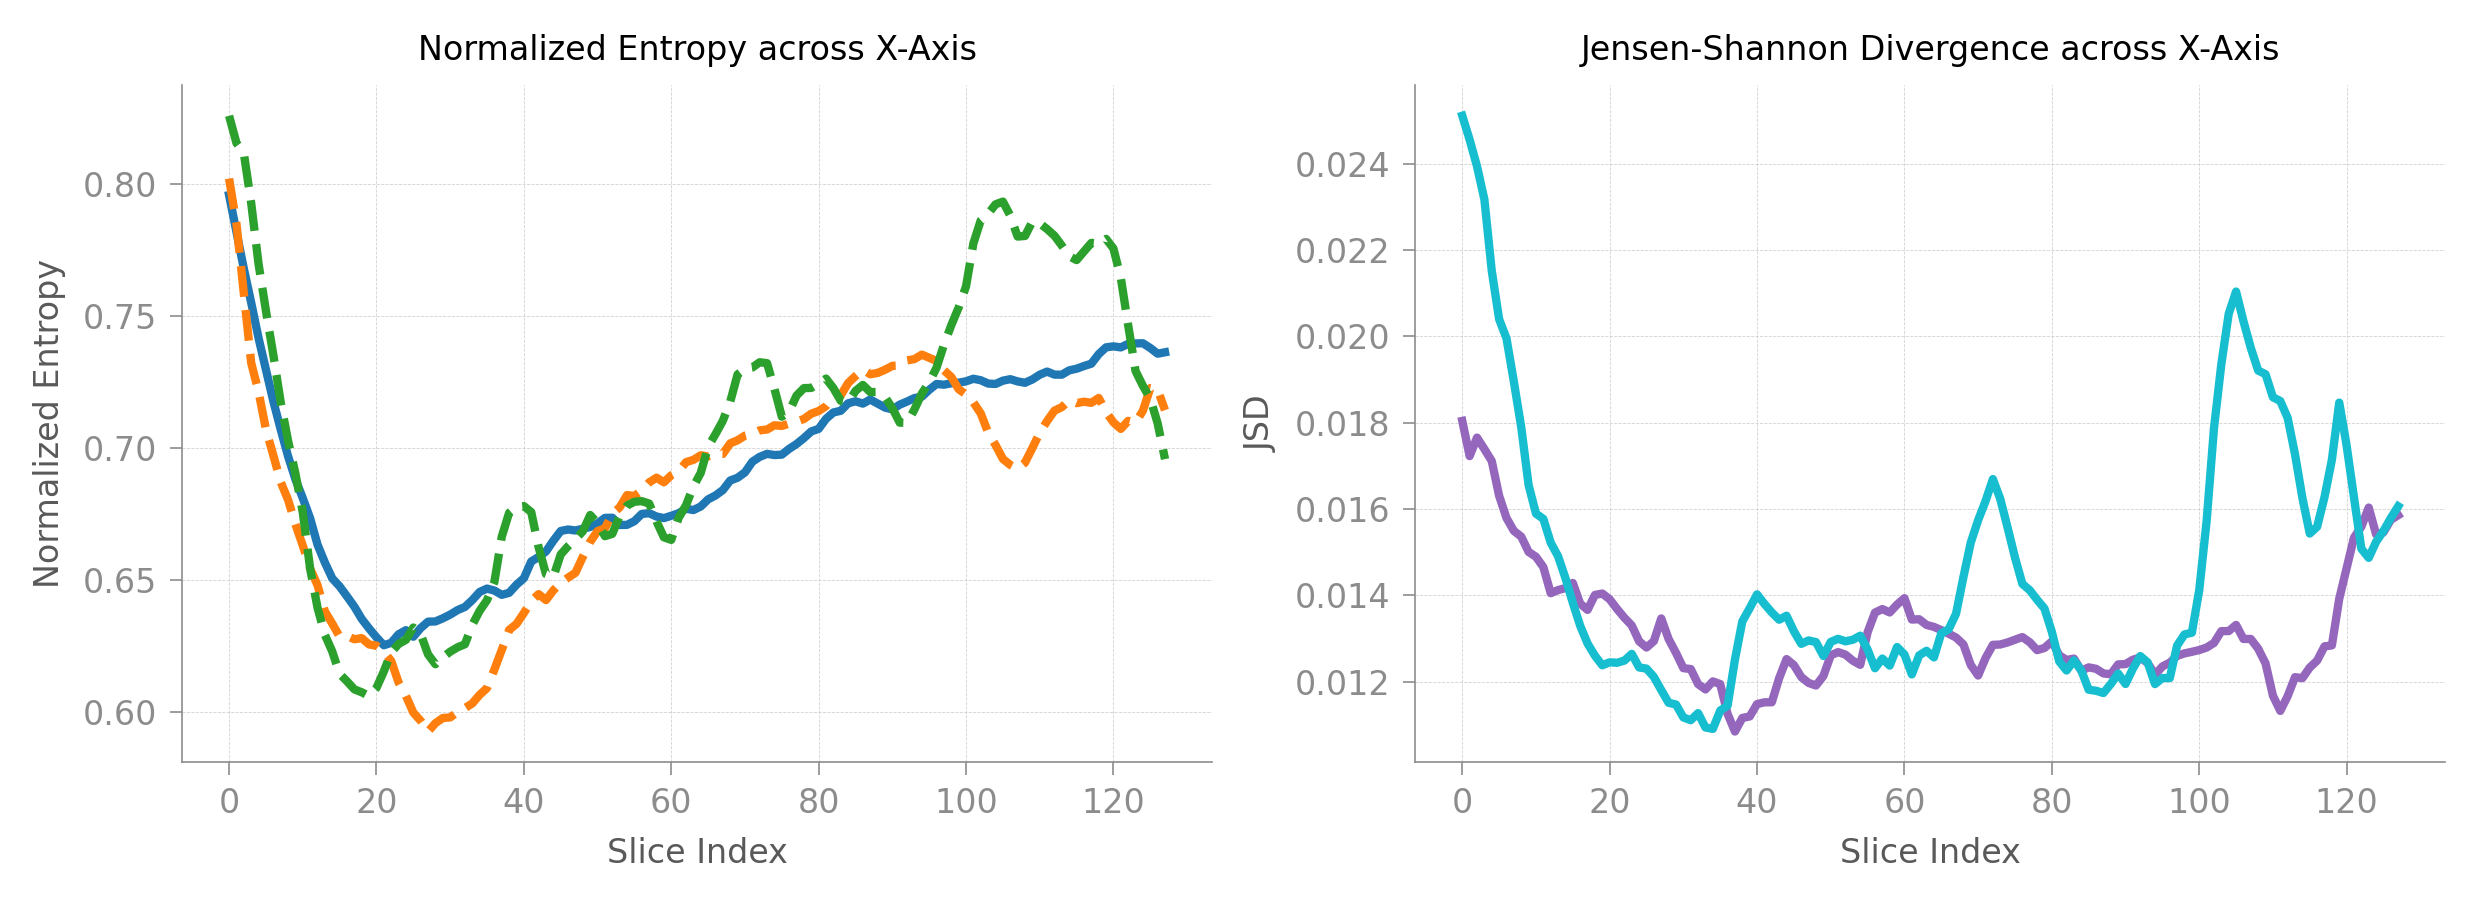
\includegraphics[width=0.9\textwidth]{figures/results/cgan_unconstrained_performance/combined_H_and_JSD_metrics_axis_X.png}
    \caption{Comparison of the \glsentryshort{jsd} normalized voxel-wise entropy across the Y, and X axes.}
    \label{fig:H_norm_over_XY_axes}
\end{figure}

\begin{figure}[htbp!]
    \centering
    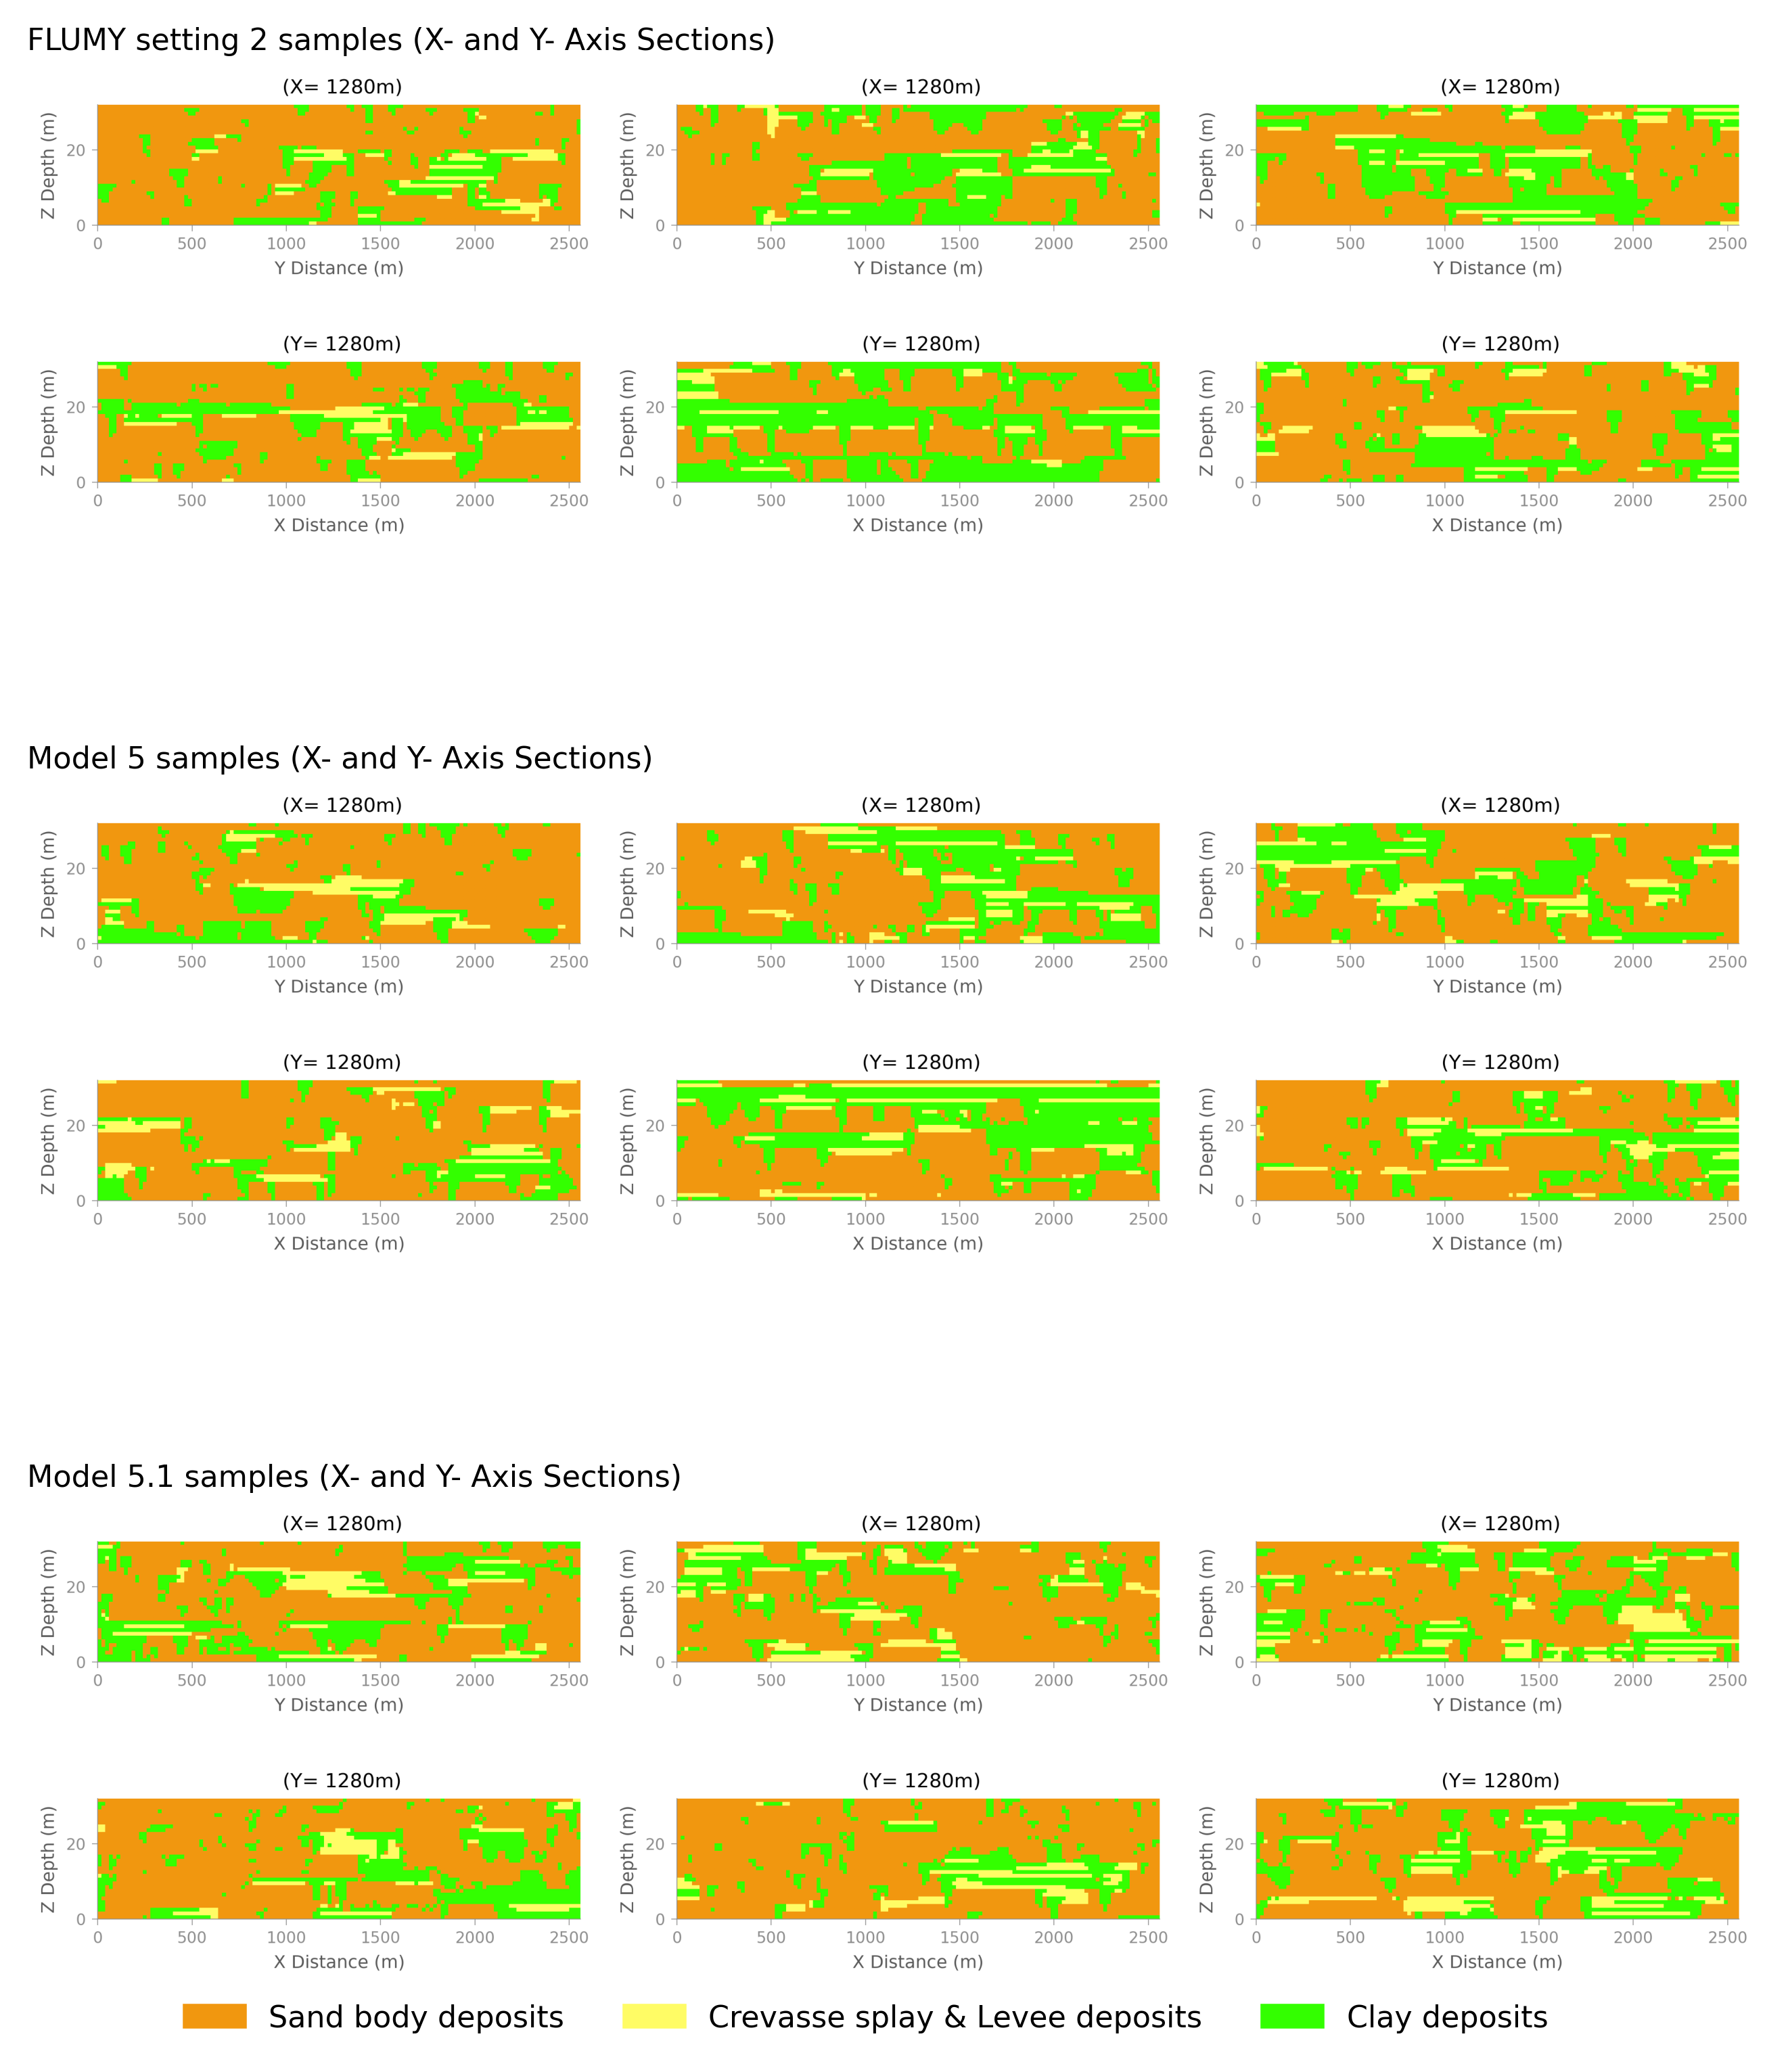
\includegraphics[width=0.99\linewidth]{figures/appendix/appendix_E/master_grouped_vertical_6x1.png}
    \caption{tba}
    \label{fig:2D_XY_slices_models_5(1)_and_flumy}
\end{figure}